\section{波动问题}
\label{sec:wave-problem}

一根弦的运动由什么决定？先从受力写出方程，看清位移、速度、波速和外力各自的位置，再讨论弦的端点能怎样约束运动。

\paragraph{从张力到方程}
设弦静止时沿$x$轴拉直，线密度（单位长度的质量）为常数$\rho>0$，张力大小为常数$\kappa>0$。记$u(x,t)$为点$x$在时刻$t$的竖直位移。我们只考虑小振动：斜率满足$\lvert\partial_xu\rvert\ll1$，弦上各点只沿竖直方向运动。

取一小段$[x,x+\Delta x]$，如图~\ref{fig:wave-string-element}。它的两端各受一个沿切线方向的张力，水平分量近似抵消，竖直分量决定这一小段的加速度。设切线与水平方向的夹角为$\theta$，则$\tan\theta=\partial_xu$，于是
\[
 \sin\theta=\frac{\partial_xu}{\sqrt{1+(\partial_xu)^{2}}}=\partial_xu+O\bigl(\lvert\partial_xu\rvert^{3}\bigr).
\]
小斜率假设在这里起作用：竖直分量可以用$\kappa\,\partial_xu$代替，弦的伸长也只是斜率的二阶量，所以张力保持常数。

\begin{BookInlineFigure}
  \centering
  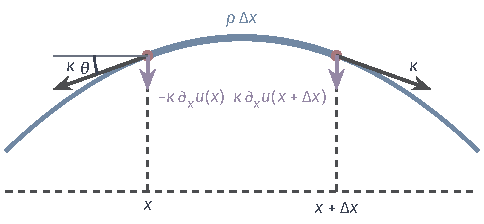
\includegraphics[width=81.975mm]{figures/06-differential-equations/02-partial-differential-equations/tikz/wave-string-element/figure.pdf}
  \caption{弦上一小段$[x,x+\Delta x]$的受力。蓝色粗线是这一小段，质量为$\rho\,\Delta x$。深灰箭头是两端沿切线的张力$\kappa$，紫色箭头是它们的竖直分量。这里弦向上凸，两个竖直分量都向下，合力把这一段拉回平衡位置。}
  \label{fig:wave-string-element}
\end{BookInlineFigure}

右端受到的竖直力是$\kappa\,\partial_xu(x+\Delta x,t)$，左端受到的是$-\kappa\,\partial_xu(x,t)$。再设单位质量上的竖直外力为$f(x,t)$。对这一小段用牛顿第二定律，得到
\[
 \rho\,\Delta x\,\partial_t^{2}u\approx\kappa\bigl[\partial_xu(x+\Delta x,t)-\partial_xu(x,t)\bigr]+\rho\,\Delta x\,f .
\]

两边除以$\rho\,\Delta x$，令$\Delta x\to0$，方括号除以$\Delta x$成为$\partial_x^{2}u$。于是得到一维波动方程：
\begin{equation}
 \partial_t^{2}u=c^{2}\partial_x^{2}u+f,\qquad c^{2}=\frac{\kappa}{\rho}.
 \label{eq:wave-string}
\end{equation}
常数$c>0$称为\term{波速}（wave speed）。量纲上$\kappa/\rho$的单位是$\mathrm{m^2/s^2}$，所以$c$确实是速度，后文会看到它正是扰动传播的速度。例如线密度$0.005\,\mathrm{kg/m}$、张力$80\,\mathrm{N}$的弦，$c=\sqrt{16000}\approx126.5\,\mathrm{m/s}$。张力越大、弦越轻，波跑得越快。

方程中的量各有含义，列在表~\ref{tab:wave-quantities}中。

\begin{BookInlineTable}
  \centering
  \caption{弦振动中各量的含义}
  \label{tab:wave-quantities}
  \begin{tabular}{lll}
    \toprule
    量 & 含义 & 在方程中的作用\\
    \midrule
    $u$ & 竖直位移 & 未知场\\
    $\partial_tu$ & 竖直速度 & 与位移一起构成状态\\
    $\partial_x^{2}u$ & 弦的弯曲 & 决定张力合力\\
    $c$ & 波速 & 把弯曲换算成加速度\\
    $f$ & 单位质量的外力 & 直接提供加速度\\
    \bottomrule
  \end{tabular}
\end{BookInlineTable}

\paragraph{弯曲决定加速度}
式~\eqref{eq:wave-string}和第~\ref{chap:diffusion-equations}章的热方程$\partial_tu=\partial_x^{2}u$右端相同，都是弯曲程度。区别只在左端：弯曲在热方程里决定变化的速度，在波动方程里决定变化的加速度。

这一个差别足以产生完全不同的运动。取初始形状$u_0=\mathrm{e}^{-x^{2}}$，$c=1$，波动问题的初速度为零。在$x=0$处，弯曲是$\partial_x^{2}u_0(0)=-2$。热方程的解在这一点的前期行为是下面左式，波动方程的解是右式：
\[
 u^{\mathrm{heat}}(0,t)\approx1-2t,\qquad u^{\mathrm{wave}}(0,t)\approx1-t^{2}.
\]

热方程中顶点一开始就以速度$2$下降，凡是向上凸的地方都立刻下降，凡是向下凹的地方都立刻上升，所以鼓包被抹平。弦的情形中，同样的弯曲只给出加速度，弦要积累速度才开始移动。一旦有了速度，弯曲消失后运动也不会停下，弦会冲过平衡位置。

图~\ref{fig:wave-curvature-acceleration}把这个差别画了出来。(a)的箭头是弯曲给出的量，(b)中热方程的鼓包逐渐变矮变宽并保持一个峰，(c)中波动方程的鼓包裂成了两个向外移动的峰。

\begin{BookInlineFigure}
  \centering
  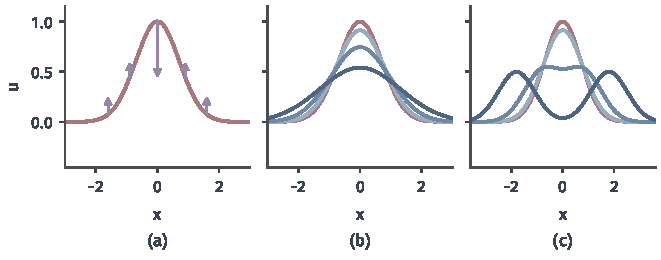
\includegraphics[width=112mm]{figures/06-differential-equations/02-partial-differential-equations/matplotlib/wave-curvature-acceleration/figure.pdf}
  \caption{同样的弯曲，两种后果。(a)初值$\mathrm{e}^{-x^{2}}$（红）和各点的弯曲$\partial_x^{2}u$（紫色箭头）。(b)热方程，蓝色由浅到深为$t=0.05,0.2,0.6$，弯曲作为速度，鼓包被抹平。(c)波动方程，$c=1$，初速度为零，蓝色由浅到深为$t=0.3,0.8,1.8$，弯曲作为加速度，鼓包裂成两个峰。}
  \label{fig:wave-curvature-acceleration}
\end{BookInlineFigure}

\paragraph{把弦看成珠链}
把函数看成很长的向量，可以把这个差别说得更具体。把弦换成$N$颗质量为$\rho h$的珠子，间距为$h$，相邻珠子之间由张力$\kappa$的轻线相连，如图~\ref{fig:wave-bead-chain}。第$j$颗珠子受到两侧的竖直拉力，分别正比于它与邻居的高度差除以$h$。

\begin{BookInlineFigure}
  \centering
  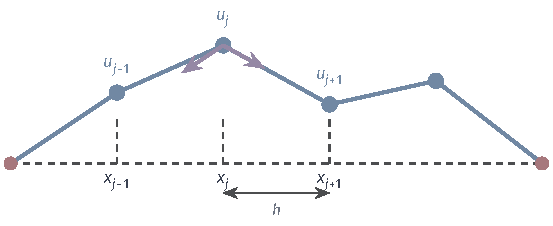
\includegraphics[width=93.606mm]{figures/06-differential-equations/02-partial-differential-equations/tikz/wave-bead-chain/figure.pdf}
  \caption{把弦换成珠链。珠子间距为$h$，两端（红点）固定。第$j$颗珠子受到两侧轻线的拉力（紫色箭头），竖直合力正比于$u_{j+1}-2u_j+u_{j-1}$，这正是二阶差分。}
  \label{fig:wave-bead-chain}
\end{BookInlineFigure}

列出第$j$颗珠子的牛顿第二定律，两端固定时取$u_0=u_{N+1}=0$，并除以质量，得到
\[
 \ddot{u}_j=c^{2}\,\frac{u_{j+1}-2u_j+u_{j-1}}{h^{2}},\qquad j=1,\ldots,N.
\]
记$\bm{u}=(u_1,\ldots,u_N)^\top$，$\bm{K}$为$h^{-2}$乘三对角矩阵$\mathrm{tridiag}(-1,2,-1)$，它对称正定。上式就是
\begin{equation}
 \ddot{\bm{u}}=-c^{2}\bm{K}\bm{u}.
 \label{eq:wave-chain}
\end{equation}

同样的空间离散用在热方程上，得到$\dot{\bm{u}}=-\bm{K}\bm{u}$。两个方程只差一阶时间导数，共用同一个矩阵$\bm{K}$。设$\bm{v}$是$\bm{K}$的特征向量，特征值为$\lambda>0$，把解限制在这个方向上，系数$a(t)$分别满足下面两个常微分方程：
\[
 \dot{a}=-\lambda a,\qquad \ddot{a}=-c^{2}\lambda a.
\]
前者给出衰减$\mathrm{e}^{-\lambda t}$，后者给出振荡$\cos(c\sqrt{\lambda}\,t)$。所以每个方向上一个是指数衰减，一个是不衰减的简谐振动，这是本章反复用到的对应。

这个类比也有失效的地方。珠链的频率有上限，这是因为特征值有上限；连续的弦可以振动得任意快。珠链上的扰动实际上以略低于$c$的速度散开，而连续弦上的波形不变。第~\ref{sec:wave-modes}节会用具体数字比较这些差别，波动方程的离散求解放在第~\ref{chap:pde-numerical-methods}章。

\paragraph{初始状态是一对函数}
式~\eqref{eq:wave-chain}的每个分量都是二阶常微分方程，要同时给位置和速度。连续的弦也一样，初始状态是一对函数：初始位移$u_0$和初始速度$u_1$。第~\ref{chap:pde-problems}章的例子正说明了这一点：$(0,1)$上$c=1$、两端固定时，$\cos(\pi t)\sin(\pi x)$和$(\cos\pi t+\sin\pi t)\sin(\pi x)$的初始位移相同，都是$\sin\pi x$，后续运动却不同。

把区域写成一般形式，本章的问题可以统一写出。

\begin{definition}[波动方程的初边值问题]
\label{def:wave-ibvp}
设$\Omega\subset\mathbb{R}^{d}$为区域，$c>0$，$T>0$。给定源项$f$、初始位移$u_0$和初始速度$u_1$。求$u(\bm{x},t)$满足
\begin{equation}
 \begin{aligned}
  \partial_t^{2}u-c^{2}\Delta u&=f && \text{于}\ \Omega\times(0,T],\\
  u(\cdot,0)=u_0,\quad\partial_tu(\cdot,0)&=u_1 && \text{于}\ \Omega,
 \end{aligned}
 \label{eq:wave-ibvp}
\end{equation}
以及边界$\partial\Omega\times(0,T]$上给定的边界条件。$\Omega=\mathbb{R}^{d}$时没有边界条件。
\end{definition}

\paragraph{端点怎样约束运动}
端点条件有两种基本类型，如图~\ref{fig:wave-boundary-types}。把弦的一端钉死，得到\term{固定端}（fixed end）$u=0$，端点没有位移，因而没有速度。把弦的一端系在一个能沿竖直光滑杆自由滑动的无质量小环上，得到\term{自由端}（free end）。小环在竖直方向不能受力，否则加速度无穷大，所以张力的竖直分量为零，即$\partial_xu=0$。

\begin{BookInlineFigure}
  \centering
  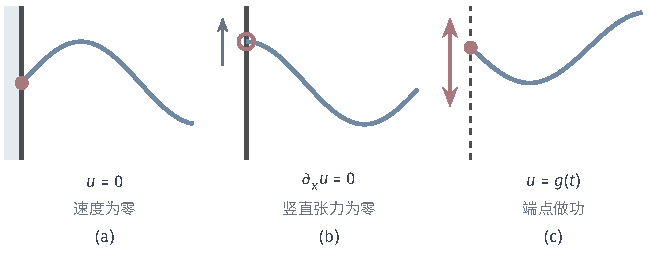
\includegraphics[width=109.703mm]{figures/06-differential-equations/02-partial-differential-equations/tikz/wave-boundary-types/figure.pdf}
  \caption{三种端点。(a)固定端：端点位移和速度为零。(b)自由端：小环沿光滑竖直杆滑动，弦在端点的切线水平。(c)驱动端：端点按给定的位移$g(t)$运动，并通过张力向弦做功。}
  \label{fig:wave-boundary-types}
\end{BookInlineFigure}

两种条件限制的量不同，共同点是端点不向弦输入能量。功率等于力乘速度。在端点上，支撑对弦的竖直力等于$\kappa\,\partial_{\bm{n}}u$，其中$\partial_{\bm{n}}$是外法向导数：右端是$\partial_x$，左端是$-\partial_x$。所以端点向弦输入的功率是
\begin{equation}
 P=\kappa\,\partial_{\bm{n}}u\,\partial_tu .
 \label{eq:wave-end-power}
\end{equation}

固定端让第二个因子$\partial_tu$为零，自由端让第一个因子$\partial_{\bm{n}}u$为零。两种方式都使$P=0$。如果端点按给定的位移运动，或者端点上施加给定的力，式~\eqref{eq:wave-end-power}一般不为零，能量就通过端点进出弦。表~\ref{tab:wave-boundary}总结了这四种情形。

\begin{BookInlineTable}
  \centering
  \caption{端点条件和端点功率}
  \label{tab:wave-boundary}
  \begin{tabular}{llll}
    \toprule
    端点 & 条件 & 被规定的量 & 功率$P$\\
    \midrule
    固定端 & $u=0$ & 位移和速度 & $0$\\
    自由端 & $\partial_{\bm{n}}u=0$ & 竖直力 & $0$\\
    位移驱动 & $u=g(t)$ & 位移和速度 & $\kappa\,\partial_{\bm{n}}u\,g'(t)$\\
    力驱动 & $\kappa\,\partial_{\bm{n}}u=g(t)$ & 竖直力 & $g(t)\,\partial_tu$\\
    \bottomrule
  \end{tabular}
\end{BookInlineTable}

初值和边值在角点处要彼此相容。位移驱动的左端$u(0,t)=g(t)$要有$C^{2}$解，必须满足下面三个条件，它们依次来自位移相等、速度相等和方程在角点处成立：
\[
 u_0(0)=g(0),\qquad u_1(0)=g'(0),\qquad g''(0)=c^{2}u_0''(0)+f(0,0).
\]
固定端是$g\equiv0$的情形。不相容时，间断或折角会从角点出发沿特征线传播，解只能在弱的意义下理解。
